% !TeX root = ../../main.tex
\section{Non-detailed reactor modelling} \label{Non-detailed}
\subsection{Kinetics of other reactions}
\subsubsection{Hydrogenation of o-nitrotoluene}
After the production of the 3 nitrotoluene isomers, (mention separation?) ONT is mixed with propanol and hydrogenated to o-TOL in a co-current trickle bed reactor operating at 333K and 3 atm. 

\begin{scheme}[h]
    \centering
    \ch{ ONT + 3 H2 -> O{-}TOL + 2 H2O }
    \caption{ONT hydrogenation to O-TOL}
    \label{eqn: ONT hydrogenation}
\end{scheme}

include ChemDraw here
The rate equation for this equation can be defined as: 
\begin{equation}
    r = k P_{H_2}^{0.3} 
    \label{ONT rate equation}
\end{equation}
 \begin{equation}
    k = 211.69 \exp \bigg(-\frac{45.52 \cdot 10^{3}}{RT}\bigg) \frac{mol}{kPa^{0.3}g_{cat}s}
 \end{equation}
 
\subsubsection{Oxidation of p-nitrotoluene}
% Andreas

\begin{scheme}[h]
    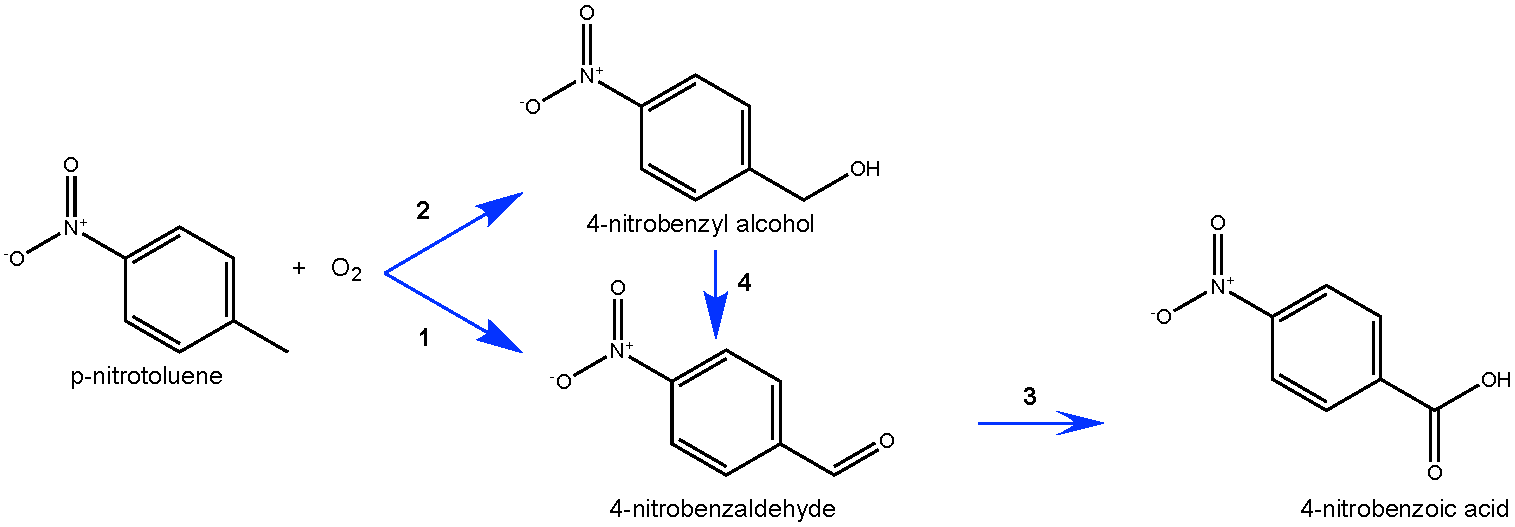
\includegraphics[width=\linewidth]{figures/R3.pdf}
    \caption{Oxidation of 4-nitrotoluene to 4-nitrobenzaldehyde, and subsequently to 4-nitrobenzoic acid}
    \label{sch:R3}
\end{scheme}

\begin{table}[h]
\centering
\begin{tabular}{@{}lS[table-format=1.3e1]S[table-format=3.2]@{}}
\toprule
Reaction & {$A$ (\si{\per\s})} & {$E_a$ (\si{\kJ\per\mol})} \\ \midrule
1        & 7.068e9  & 123.91      \\
2        & 1.503e3  & 69.54       \\
3        & 5.621e4  & 66.84       \\
4        & 3.384e6  & 81.27       \\ \bottomrule
\end{tabular}
\end{table}

\subsubsection{Hydrogenation of nitrobenzaldehyde and nitrobenzoic acid}

\begin{scheme}[h]
    \centering
    \ch{ NBA + HCOOH -> ABA + CO2 + H2O }
    \\
    \ch{ NBAH + HCOOH -> ABAH + CO2 + H2O }
    \caption{Hydrogenation of NBA and NBAH to ABA and ABAH}
    \label{eqn: ONT hydrogenation}
\end{scheme}

The hydrogenation of p-nitrobenzaldehyde and p-nitrobenzoic acid were carried out in methanol solvent with formic acid as the reducing agent. The reaction was carried out at room temperature and 1 atm. 5\% w/w Pt/C was chosen as the desired catalyst to speed up the reaction because it can be reused many times while maintaining its catalytic performance \cite{rahman_fast_2020}. The overall yield for 4-ABA and 4-ABH are 86\% and 80\% respectively as reported in [gowda and mahesh].

\subsection{Summary of reactor specification}
The reactors were chosen on the basis of safety and performance. For the hydrogenation of ONT, a co-current trickle bed reactor was chosen due to the high conversion performanceFull detailed analysis for each reactor choice can be found in \ref{sec:reactorchoices}.